% Created by tikzDevice version 0.12.6 on 2026-07-06 23:55:44
% !TEX encoding = UTF-8 Unicode
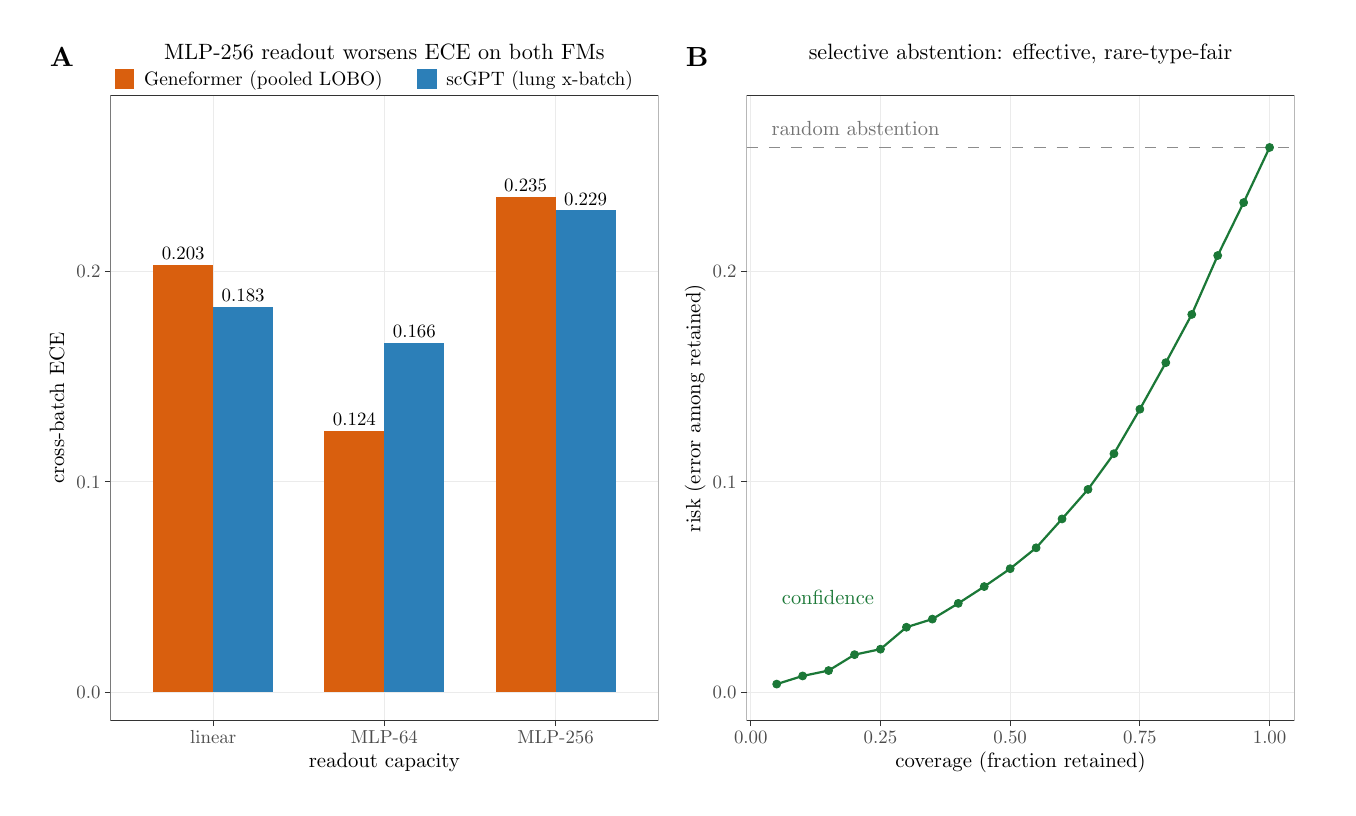
\begin{tikzpicture}[x=1pt,y=1pt]
\definecolor{fillColor}{RGB}{255,255,255}
\path[use as bounding box,fill=fillColor,fill opacity=0.00] (0,0) rectangle (469.75,274.63);
\begin{scope}
\path[clip] (  0.00,  0.00) rectangle (469.75,274.63);
\definecolor{drawColor}{RGB}{255,255,255}
\definecolor{fillColor}{RGB}{255,255,255}

\path[draw=drawColor,line width= 0.4pt,line join=round,line cap=round,fill=fillColor] ( -0.00,  0.00) rectangle (469.76,274.63);
\end{scope}
\begin{scope}
\path[clip] (  4.00,  3.00) rectangle (233.88,271.63);
\definecolor{drawColor}{RGB}{255,255,255}
\definecolor{fillColor}{RGB}{255,255,255}

\path[draw=drawColor,line width= 0.4pt,line join=round,line cap=round,fill=fillColor] (  4.00,  3.00) rectangle (233.88,271.63);
\end{scope}
\begin{scope}
\path[clip] (233.88,  3.00) rectangle (463.76,271.63);
\definecolor{drawColor}{RGB}{255,255,255}
\definecolor{fillColor}{RGB}{255,255,255}

\path[draw=drawColor,line width= 0.4pt,line join=round,line cap=round,fill=fillColor] (233.88,  3.00) rectangle (463.75,271.63);
\end{scope}
\begin{scope}
\path[clip] ( 29.91, 24.23) rectangle (227.88,250.06);
\definecolor{fillColor}{RGB}{255,255,255}

\path[fill=fillColor] ( 29.91, 24.23) rectangle (227.88,250.06);
\definecolor{drawColor}{gray}{0.92}

\path[draw=drawColor,line width= 0.4pt,line join=round] ( 29.91, 34.49) --
	(227.88, 34.49);

\path[draw=drawColor,line width= 0.4pt,line join=round] ( 29.91,110.53) --
	(227.88,110.53);

\path[draw=drawColor,line width= 0.4pt,line join=round] ( 29.91,186.57) --
	(227.88,186.57);

\path[draw=drawColor,line width= 0.4pt,line join=round] ( 67.03, 24.23) --
	( 67.03,250.06);

\path[draw=drawColor,line width= 0.4pt,line join=round] (128.89, 24.23) --
	(128.89,250.06);

\path[draw=drawColor,line width= 0.4pt,line join=round] (190.76, 24.23) --
	(190.76,250.06);
\definecolor{fillColor}{RGB}{44,127,184}

\path[fill=fillColor] ( 67.03, 34.49) rectangle ( 88.68,173.64);

\path[fill=fillColor] (128.89, 34.49) rectangle (150.55,160.72);

\path[fill=fillColor] (190.76, 34.49) rectangle (212.41,208.62);
\definecolor{fillColor}{RGB}{217,95,14}

\path[fill=fillColor] ( 45.38, 34.49) rectangle ( 67.03,188.93);

\path[fill=fillColor] (107.24, 34.49) rectangle (128.89,128.93);

\path[fill=fillColor] (169.11, 34.49) rectangle (190.76,213.56);
\definecolor{drawColor}{RGB}{0,0,0}

\node[text=drawColor,anchor=base,inner sep=0pt, outer sep=0pt, scale=  0.68] at ( 77.86,175.52) {0.183};

\node[text=drawColor,anchor=base,inner sep=0pt, outer sep=0pt, scale=  0.68] at (139.72,162.60) {0.166};

\node[text=drawColor,anchor=base,inner sep=0pt, outer sep=0pt, scale=  0.68] at (201.58,210.50) {0.229};

\node[text=drawColor,anchor=base,inner sep=0pt, outer sep=0pt, scale=  0.68] at ( 56.20,190.81) {0.203};

\node[text=drawColor,anchor=base,inner sep=0pt, outer sep=0pt, scale=  0.68] at (118.07,130.81) {0.124};

\node[text=drawColor,anchor=base,inner sep=0pt, outer sep=0pt, scale=  0.68] at (179.93,215.44) {0.235};
\definecolor{drawColor}{gray}{0.20}

\path[draw=drawColor,line width= 0.4pt,line join=round,line cap=round] ( 29.91, 24.23) rectangle (227.88,250.06);
\end{scope}
\begin{scope}
\path[clip] (  0.00,  0.00) rectangle (469.75,274.63);
\definecolor{drawColor}{gray}{0.30}

\node[text=drawColor,anchor=base east,inner sep=0pt, outer sep=0pt, scale=  0.68] at ( 26.31, 32.15) {0.0};

\node[text=drawColor,anchor=base east,inner sep=0pt, outer sep=0pt, scale=  0.68] at ( 26.31,108.19) {0.1};

\node[text=drawColor,anchor=base east,inner sep=0pt, outer sep=0pt, scale=  0.68] at ( 26.31,184.23) {0.2};
\end{scope}
\begin{scope}
\path[clip] (  0.00,  0.00) rectangle (469.75,274.63);
\definecolor{drawColor}{gray}{0.20}

\path[draw=drawColor,line width= 0.4pt,line join=round] ( 27.91, 34.49) --
	( 29.91, 34.49);

\path[draw=drawColor,line width= 0.4pt,line join=round] ( 27.91,110.53) --
	( 29.91,110.53);

\path[draw=drawColor,line width= 0.4pt,line join=round] ( 27.91,186.57) --
	( 29.91,186.57);
\end{scope}
\begin{scope}
\path[clip] (  0.00,  0.00) rectangle (469.75,274.63);
\definecolor{drawColor}{gray}{0.20}

\path[draw=drawColor,line width= 0.4pt,line join=round] ( 67.03, 22.23) --
	( 67.03, 24.23);

\path[draw=drawColor,line width= 0.4pt,line join=round] (128.89, 22.23) --
	(128.89, 24.23);

\path[draw=drawColor,line width= 0.4pt,line join=round] (190.76, 22.23) --
	(190.76, 24.23);
\end{scope}
\begin{scope}
\path[clip] (  0.00,  0.00) rectangle (469.75,274.63);
\definecolor{drawColor}{gray}{0.30}

\node[text=drawColor,anchor=base,inner sep=0pt, outer sep=0pt, scale=  0.68] at ( 67.03, 15.95) {linear};

\node[text=drawColor,anchor=base,inner sep=0pt, outer sep=0pt, scale=  0.68] at (128.89, 15.95) {MLP-64};

\node[text=drawColor,anchor=base,inner sep=0pt, outer sep=0pt, scale=  0.68] at (190.76, 15.95) {MLP-256};
\end{scope}
\begin{scope}
\path[clip] (  0.00,  0.00) rectangle (469.75,274.63);
\definecolor{drawColor}{RGB}{0,0,0}

\node[text=drawColor,anchor=base,inner sep=0pt, outer sep=0pt, scale=  0.75] at (128.89,  7.46) {readout capacity};
\end{scope}
\begin{scope}
\path[clip] (  0.00,  0.00) rectangle (469.75,274.63);
\definecolor{drawColor}{RGB}{0,0,0}

\node[text=drawColor,rotate= 90.00,anchor=base,inner sep=0pt, outer sep=0pt, scale=  0.75] at ( 13.17,137.14) {cross-batch ECE};
\end{scope}
\begin{scope}
\path[clip] (  0.00,  0.00) rectangle (469.75,274.63);
\definecolor{fillColor}{RGB}{255,255,255}

\path[fill=fillColor] ( 30.07,252.06) rectangle (227.72,260.06);
\end{scope}
\begin{scope}
\path[clip] (  0.00,  0.00) rectangle (469.75,274.63);
\definecolor{fillColor}{RGB}{255,255,255}

\path[fill=fillColor] ( 31.07,252.06) rectangle ( 39.07,260.06);
\definecolor{fillColor}{RGB}{217,95,14}

\path[fill=fillColor] ( 31.59,252.58) rectangle ( 38.55,259.54);
\end{scope}
\begin{scope}
\path[clip] (  0.00,  0.00) rectangle (469.75,274.63);
\definecolor{fillColor}{RGB}{255,255,255}

\path[fill=fillColor] (140.27,252.06) rectangle (148.27,260.06);
\definecolor{fillColor}{RGB}{44,127,184}

\path[fill=fillColor] (140.79,252.58) rectangle (147.76,259.54);
\end{scope}
\begin{scope}
\path[clip] (  0.00,  0.00) rectangle (469.75,274.63);
\definecolor{drawColor}{RGB}{0,0,0}

\node[text=drawColor,anchor=base west,inner sep=0pt, outer sep=0pt, scale=  0.70] at ( 42.07,253.65) {Geneformer (pooled LOBO)};
\end{scope}
\begin{scope}
\path[clip] (  0.00,  0.00) rectangle (469.75,274.63);
\definecolor{drawColor}{RGB}{0,0,0}

\node[text=drawColor,anchor=base west,inner sep=0pt, outer sep=0pt, scale=  0.70] at (151.27,253.65) {scGPT (lung x-batch)};
\end{scope}
\begin{scope}
\path[clip] (  0.00,  0.00) rectangle (469.75,274.63);
\definecolor{drawColor}{RGB}{0,0,0}

\node[text=drawColor,anchor=base,inner sep=0pt, outer sep=0pt, scale=  0.80] at (128.89,263.12) {MLP-256 readout worsens ECE on both FMs};
\end{scope}
\begin{scope}
\path[clip] (  0.00,  0.00) rectangle (469.75,274.63);
\definecolor{drawColor}{RGB}{0,0,0}

\node[text=drawColor,anchor=base,inner sep=0pt, outer sep=0pt, scale=  1.00] at ( 12.35,260.75) {\bfseries A};
\end{scope}
\begin{scope}
\path[clip] (259.79, 24.23) rectangle (457.76,250.06);
\definecolor{fillColor}{RGB}{255,255,255}

\path[fill=fillColor] (259.79, 24.23) rectangle (457.75,250.06);
\definecolor{drawColor}{gray}{0.92}

\path[draw=drawColor,line width= 0.4pt,line join=round] (259.79, 34.49) --
	(457.76, 34.49);

\path[draw=drawColor,line width= 0.4pt,line join=round] (259.79,110.53) --
	(457.76,110.53);

\path[draw=drawColor,line width= 0.4pt,line join=round] (259.79,186.57) --
	(457.76,186.57);

\path[draw=drawColor,line width= 0.4pt,line join=round] (261.29, 24.23) --
	(261.29,250.06);

\path[draw=drawColor,line width= 0.4pt,line join=round] (308.15, 24.23) --
	(308.15,250.06);

\path[draw=drawColor,line width= 0.4pt,line join=round] (355.02, 24.23) --
	(355.02,250.06);

\path[draw=drawColor,line width= 0.4pt,line join=round] (401.89, 24.23) --
	(401.89,250.06);

\path[draw=drawColor,line width= 0.4pt,line join=round] (448.76, 24.23) --
	(448.76,250.06);
\definecolor{drawColor}{gray}{0.55}

\path[draw=drawColor,line width= 0.4pt,dash pattern=on 4pt off 4pt ,line join=round] (259.79,231.36) -- (457.76,231.36);
\definecolor{drawColor}{gray}{0.45}

\node[text=drawColor,anchor=base west,inner sep=0pt, outer sep=0pt, scale=  0.74] at (268.79,235.65) {random abstention};
\definecolor{drawColor}{RGB}{27,120,55}

\path[draw=drawColor,line width= 0.8pt,line join=round] (270.66, 37.43) --
	(280.03, 40.37) --
	(289.41, 42.32) --
	(298.78, 48.07) --
	(308.15, 50.05) --
	(317.53, 57.98) --
	(326.90, 60.92) --
	(336.27, 66.60) --
	(345.65, 72.67) --
	(355.02, 79.13) --
	(364.40, 86.68) --
	(373.77, 97.12) --
	(383.14,107.78) --
	(392.52,120.69) --
	(401.89,136.76) --
	(411.26,153.58) --
	(420.64,171.01) --
	(430.01,192.29) --
	(439.38,211.42) --
	(448.76,231.34);
\definecolor{fillColor}{RGB}{27,120,55}

\path[draw=drawColor,line width= 0.3pt,line join=round,line cap=round,fill=fillColor] (270.66, 37.43) circle (  1.44);

\path[draw=drawColor,line width= 0.3pt,line join=round,line cap=round,fill=fillColor] (280.03, 40.37) circle (  1.44);

\path[draw=drawColor,line width= 0.3pt,line join=round,line cap=round,fill=fillColor] (289.41, 42.32) circle (  1.44);

\path[draw=drawColor,line width= 0.3pt,line join=round,line cap=round,fill=fillColor] (298.78, 48.07) circle (  1.44);

\path[draw=drawColor,line width= 0.3pt,line join=round,line cap=round,fill=fillColor] (308.15, 50.05) circle (  1.44);

\path[draw=drawColor,line width= 0.3pt,line join=round,line cap=round,fill=fillColor] (317.53, 57.98) circle (  1.44);

\path[draw=drawColor,line width= 0.3pt,line join=round,line cap=round,fill=fillColor] (326.90, 60.92) circle (  1.44);

\path[draw=drawColor,line width= 0.3pt,line join=round,line cap=round,fill=fillColor] (336.27, 66.60) circle (  1.44);

\path[draw=drawColor,line width= 0.3pt,line join=round,line cap=round,fill=fillColor] (345.65, 72.67) circle (  1.44);

\path[draw=drawColor,line width= 0.3pt,line join=round,line cap=round,fill=fillColor] (355.02, 79.13) circle (  1.44);

\path[draw=drawColor,line width= 0.3pt,line join=round,line cap=round,fill=fillColor] (364.40, 86.68) circle (  1.44);

\path[draw=drawColor,line width= 0.3pt,line join=round,line cap=round,fill=fillColor] (373.77, 97.12) circle (  1.44);

\path[draw=drawColor,line width= 0.3pt,line join=round,line cap=round,fill=fillColor] (383.14,107.78) circle (  1.44);

\path[draw=drawColor,line width= 0.3pt,line join=round,line cap=round,fill=fillColor] (392.52,120.69) circle (  1.44);

\path[draw=drawColor,line width= 0.3pt,line join=round,line cap=round,fill=fillColor] (401.89,136.76) circle (  1.44);

\path[draw=drawColor,line width= 0.3pt,line join=round,line cap=round,fill=fillColor] (411.26,153.58) circle (  1.44);

\path[draw=drawColor,line width= 0.3pt,line join=round,line cap=round,fill=fillColor] (420.64,171.01) circle (  1.44);

\path[draw=drawColor,line width= 0.3pt,line join=round,line cap=round,fill=fillColor] (430.01,192.29) circle (  1.44);

\path[draw=drawColor,line width= 0.3pt,line join=round,line cap=round,fill=fillColor] (439.38,211.42) circle (  1.44);

\path[draw=drawColor,line width= 0.3pt,line join=round,line cap=round,fill=fillColor] (448.76,231.34) circle (  1.44);

\node[text=drawColor,anchor=base west,inner sep=0pt, outer sep=0pt, scale=  0.74] at (272.54, 66.16) {confidence};
\definecolor{drawColor}{gray}{0.20}

\path[draw=drawColor,line width= 0.4pt,line join=round,line cap=round] (259.79, 24.23) rectangle (457.75,250.06);
\end{scope}
\begin{scope}
\path[clip] (  0.00,  0.00) rectangle (469.75,274.63);
\definecolor{drawColor}{gray}{0.30}

\node[text=drawColor,anchor=base east,inner sep=0pt, outer sep=0pt, scale=  0.68] at (256.19, 32.15) {0.0};

\node[text=drawColor,anchor=base east,inner sep=0pt, outer sep=0pt, scale=  0.68] at (256.19,108.19) {0.1};

\node[text=drawColor,anchor=base east,inner sep=0pt, outer sep=0pt, scale=  0.68] at (256.19,184.23) {0.2};
\end{scope}
\begin{scope}
\path[clip] (  0.00,  0.00) rectangle (469.75,274.63);
\definecolor{drawColor}{gray}{0.20}

\path[draw=drawColor,line width= 0.4pt,line join=round] (257.79, 34.49) --
	(259.79, 34.49);

\path[draw=drawColor,line width= 0.4pt,line join=round] (257.79,110.53) --
	(259.79,110.53);

\path[draw=drawColor,line width= 0.4pt,line join=round] (257.79,186.57) --
	(259.79,186.57);
\end{scope}
\begin{scope}
\path[clip] (  0.00,  0.00) rectangle (469.75,274.63);
\definecolor{drawColor}{gray}{0.20}

\path[draw=drawColor,line width= 0.4pt,line join=round] (261.29, 22.23) --
	(261.29, 24.23);

\path[draw=drawColor,line width= 0.4pt,line join=round] (308.15, 22.23) --
	(308.15, 24.23);

\path[draw=drawColor,line width= 0.4pt,line join=round] (355.02, 22.23) --
	(355.02, 24.23);

\path[draw=drawColor,line width= 0.4pt,line join=round] (401.89, 22.23) --
	(401.89, 24.23);

\path[draw=drawColor,line width= 0.4pt,line join=round] (448.76, 22.23) --
	(448.76, 24.23);
\end{scope}
\begin{scope}
\path[clip] (  0.00,  0.00) rectangle (469.75,274.63);
\definecolor{drawColor}{gray}{0.30}

\node[text=drawColor,anchor=base,inner sep=0pt, outer sep=0pt, scale=  0.68] at (261.29, 15.95) {0.00};

\node[text=drawColor,anchor=base,inner sep=0pt, outer sep=0pt, scale=  0.68] at (308.15, 15.95) {0.25};

\node[text=drawColor,anchor=base,inner sep=0pt, outer sep=0pt, scale=  0.68] at (355.02, 15.95) {0.50};

\node[text=drawColor,anchor=base,inner sep=0pt, outer sep=0pt, scale=  0.68] at (401.89, 15.95) {0.75};

\node[text=drawColor,anchor=base,inner sep=0pt, outer sep=0pt, scale=  0.68] at (448.76, 15.95) {1.00};
\end{scope}
\begin{scope}
\path[clip] (  0.00,  0.00) rectangle (469.75,274.63);
\definecolor{drawColor}{RGB}{0,0,0}

\node[text=drawColor,anchor=base,inner sep=0pt, outer sep=0pt, scale=  0.75] at (358.77,  7.46) {coverage (fraction retained)};
\end{scope}
\begin{scope}
\path[clip] (  0.00,  0.00) rectangle (469.75,274.63);
\definecolor{drawColor}{RGB}{0,0,0}

\node[text=drawColor,rotate= 90.00,anchor=base,inner sep=0pt, outer sep=0pt, scale=  0.75] at (243.04,137.14) {risk (error among retained)};
\end{scope}
\begin{scope}
\path[clip] (  0.00,  0.00) rectangle (469.75,274.63);
\definecolor{drawColor}{RGB}{0,0,0}

\node[text=drawColor,anchor=base,inner sep=0pt, outer sep=0pt, scale=  0.80] at (358.77,263.12) {selective abstention: effective, rare-type-fair};
\end{scope}
\begin{scope}
\path[clip] (  0.00,  0.00) rectangle (469.75,274.63);
\definecolor{drawColor}{RGB}{0,0,0}

\node[text=drawColor,anchor=base,inner sep=0pt, outer sep=0pt, scale=  1.00] at (241.97,260.75) {\bfseries B};
\end{scope}
\end{tikzpicture}
